% Options for packages loaded elsewhere
\PassOptionsToPackage{unicode}{hyperref}
\PassOptionsToPackage{hyphens}{url}
%
\documentclass[
]{article}
\usepackage{amsmath,amssymb}
\usepackage{iftex}
\ifPDFTeX
  \usepackage[T1]{fontenc}
  \usepackage[utf8]{inputenc}
  \usepackage{textcomp} % provide euro and other symbols
\else % if luatex or xetex
  \usepackage{unicode-math} % this also loads fontspec
  \defaultfontfeatures{Scale=MatchLowercase}
  \defaultfontfeatures[\rmfamily]{Ligatures=TeX,Scale=1}
\fi
\usepackage{lmodern}
\ifPDFTeX\else
  % xetex/luatex font selection
\fi
% Use upquote if available, for straight quotes in verbatim environments
\IfFileExists{upquote.sty}{\usepackage{upquote}}{}
\IfFileExists{microtype.sty}{% use microtype if available
  \usepackage[]{microtype}
  \UseMicrotypeSet[protrusion]{basicmath} % disable protrusion for tt fonts
}{}
\makeatletter
\@ifundefined{KOMAClassName}{% if non-KOMA class
  \IfFileExists{parskip.sty}{%
    \usepackage{parskip}
  }{% else
    \setlength{\parindent}{0pt}
    \setlength{\parskip}{6pt plus 2pt minus 1pt}}
}{% if KOMA class
  \KOMAoptions{parskip=half}}
\makeatother
\usepackage{xcolor}
\usepackage[margin=1in]{geometry}
\usepackage{color}
\usepackage{fancyvrb}
\newcommand{\VerbBar}{|}
\newcommand{\VERB}{\Verb[commandchars=\\\{\}]}
\DefineVerbatimEnvironment{Highlighting}{Verbatim}{commandchars=\\\{\}}
% Add ',fontsize=\small' for more characters per line
\usepackage{framed}
\definecolor{shadecolor}{RGB}{248,248,248}
\newenvironment{Shaded}{\begin{snugshade}}{\end{snugshade}}
\newcommand{\AlertTok}[1]{\textcolor[rgb]{0.94,0.16,0.16}{#1}}
\newcommand{\AnnotationTok}[1]{\textcolor[rgb]{0.56,0.35,0.01}{\textbf{\textit{#1}}}}
\newcommand{\AttributeTok}[1]{\textcolor[rgb]{0.13,0.29,0.53}{#1}}
\newcommand{\BaseNTok}[1]{\textcolor[rgb]{0.00,0.00,0.81}{#1}}
\newcommand{\BuiltInTok}[1]{#1}
\newcommand{\CharTok}[1]{\textcolor[rgb]{0.31,0.60,0.02}{#1}}
\newcommand{\CommentTok}[1]{\textcolor[rgb]{0.56,0.35,0.01}{\textit{#1}}}
\newcommand{\CommentVarTok}[1]{\textcolor[rgb]{0.56,0.35,0.01}{\textbf{\textit{#1}}}}
\newcommand{\ConstantTok}[1]{\textcolor[rgb]{0.56,0.35,0.01}{#1}}
\newcommand{\ControlFlowTok}[1]{\textcolor[rgb]{0.13,0.29,0.53}{\textbf{#1}}}
\newcommand{\DataTypeTok}[1]{\textcolor[rgb]{0.13,0.29,0.53}{#1}}
\newcommand{\DecValTok}[1]{\textcolor[rgb]{0.00,0.00,0.81}{#1}}
\newcommand{\DocumentationTok}[1]{\textcolor[rgb]{0.56,0.35,0.01}{\textbf{\textit{#1}}}}
\newcommand{\ErrorTok}[1]{\textcolor[rgb]{0.64,0.00,0.00}{\textbf{#1}}}
\newcommand{\ExtensionTok}[1]{#1}
\newcommand{\FloatTok}[1]{\textcolor[rgb]{0.00,0.00,0.81}{#1}}
\newcommand{\FunctionTok}[1]{\textcolor[rgb]{0.13,0.29,0.53}{\textbf{#1}}}
\newcommand{\ImportTok}[1]{#1}
\newcommand{\InformationTok}[1]{\textcolor[rgb]{0.56,0.35,0.01}{\textbf{\textit{#1}}}}
\newcommand{\KeywordTok}[1]{\textcolor[rgb]{0.13,0.29,0.53}{\textbf{#1}}}
\newcommand{\NormalTok}[1]{#1}
\newcommand{\OperatorTok}[1]{\textcolor[rgb]{0.81,0.36,0.00}{\textbf{#1}}}
\newcommand{\OtherTok}[1]{\textcolor[rgb]{0.56,0.35,0.01}{#1}}
\newcommand{\PreprocessorTok}[1]{\textcolor[rgb]{0.56,0.35,0.01}{\textit{#1}}}
\newcommand{\RegionMarkerTok}[1]{#1}
\newcommand{\SpecialCharTok}[1]{\textcolor[rgb]{0.81,0.36,0.00}{\textbf{#1}}}
\newcommand{\SpecialStringTok}[1]{\textcolor[rgb]{0.31,0.60,0.02}{#1}}
\newcommand{\StringTok}[1]{\textcolor[rgb]{0.31,0.60,0.02}{#1}}
\newcommand{\VariableTok}[1]{\textcolor[rgb]{0.00,0.00,0.00}{#1}}
\newcommand{\VerbatimStringTok}[1]{\textcolor[rgb]{0.31,0.60,0.02}{#1}}
\newcommand{\WarningTok}[1]{\textcolor[rgb]{0.56,0.35,0.01}{\textbf{\textit{#1}}}}
\usepackage{graphicx}
\makeatletter
\def\maxwidth{\ifdim\Gin@nat@width>\linewidth\linewidth\else\Gin@nat@width\fi}
\def\maxheight{\ifdim\Gin@nat@height>\textheight\textheight\else\Gin@nat@height\fi}
\makeatother
% Scale images if necessary, so that they will not overflow the page
% margins by default, and it is still possible to overwrite the defaults
% using explicit options in \includegraphics[width, height, ...]{}
\setkeys{Gin}{width=\maxwidth,height=\maxheight,keepaspectratio}
% Set default figure placement to htbp
\makeatletter
\def\fps@figure{htbp}
\makeatother
\setlength{\emergencystretch}{3em} % prevent overfull lines
\providecommand{\tightlist}{%
  \setlength{\itemsep}{0pt}\setlength{\parskip}{0pt}}
\setcounter{secnumdepth}{5}
\usepackage{booktabs}
\usepackage{longtable}
\usepackage{array}
\usepackage{multirow}
\usepackage[table]{xcolor}
\usepackage{float}
\usepackage{booktabs}
\usepackage{longtable}
\usepackage{array}
\usepackage{multirow}
\usepackage{wrapfig}
\usepackage{float}
\usepackage{colortbl}
\usepackage{pdflscape}
\usepackage{tabu}
\usepackage{threeparttable}
\usepackage{threeparttablex}
\usepackage[normalem]{ulem}
\usepackage{makecell}
\usepackage{xcolor}
\ifLuaTeX
  \usepackage{selnolig}  % disable illegal ligatures
\fi
\usepackage{bookmark}
\IfFileExists{xurl.sty}{\usepackage{xurl}}{} % add URL line breaks if available
\urlstyle{same}
\hypersetup{
  pdftitle={Impact of PM2.5 Exposure on Low Birth Weight in Ulaanbaatar (2016--2025)},
  pdfauthor={Ahmedi, Barua, Bhuyan, Karayel},
  hidelinks,
  pdfcreator={LaTeX via pandoc}}

\title{Impact of PM2.5 Exposure on Low Birth Weight in Ulaanbaatar
(2016--2025)}
\author{Ahmedi, Barua, Bhuyan, Karayel}
\date{2025-04-29}

\begin{document}
\maketitle

{
\setcounter{tocdepth}{2}
\tableofcontents
}
\begin{Shaded}
\begin{Highlighting}[]
\NormalTok{knitr}\SpecialCharTok{::}\NormalTok{opts\_knit}\SpecialCharTok{$}\FunctionTok{set}\NormalTok{(}\AttributeTok{root.dir =}\NormalTok{ here}\SpecialCharTok{::}\FunctionTok{here}\NormalTok{())}
\end{Highlighting}
\end{Shaded}

\newpage
\listoftables
\newpage
\listoffigures
\newpage

\section{Rationale and Research
Questions}\label{rationale-and-research-questions}

\newpage

\section{Dataset Information}\label{dataset-information}

\begin{Shaded}
\begin{Highlighting}[]
\CommentTok{\# Read birth weight and live births data}
\NormalTok{birth\_weight\_low }\OtherTok{\textless{}{-}} \FunctionTok{read.csv}\NormalTok{(}\FunctionTok{here}\NormalTok{(}\StringTok{"Data/Raw/BIRTH WEIGTH LOWER THAN 2500 GRAMS.csv"}\NormalTok{), }\AttributeTok{stringsAsFactors =} \ConstantTok{TRUE}\NormalTok{)}

\NormalTok{live\_births }\OtherTok{\textless{}{-}} \FunctionTok{read.csv}\NormalTok{(}\FunctionTok{here}\NormalTok{(}\StringTok{"./Data/Raw/LIVE BIRTHS.csv"}\NormalTok{), }\AttributeTok{stringsAsFactors =} \ConstantTok{TRUE}\NormalTok{)}

\CommentTok{\# Clean live births}
\NormalTok{live\_births\_clean }\OtherTok{\textless{}{-}}\NormalTok{ live\_births}
\ControlFlowTok{for}\NormalTok{ (col }\ControlFlowTok{in} \FunctionTok{names}\NormalTok{(live\_births\_clean)[}\SpecialCharTok{{-}}\DecValTok{1}\NormalTok{]) \{}
\NormalTok{  live\_births\_clean[[col]] }\OtherTok{\textless{}{-}} \FunctionTok{as.numeric}\NormalTok{(}\FunctionTok{gsub}\NormalTok{(}\StringTok{","}\NormalTok{, }\StringTok{""}\NormalTok{, live\_births\_clean[[col]]))}
\NormalTok{\}}

\CommentTok{\# Convert wide to long format}
\NormalTok{birth\_weight\_low\_long }\OtherTok{\textless{}{-}}\NormalTok{ birth\_weight\_low }\SpecialCharTok{\%\textgreater{}\%} 
  \FunctionTok{pivot\_longer}\NormalTok{(}\SpecialCharTok{{-}}\NormalTok{Aimag, }\AttributeTok{names\_to =} \StringTok{"Month"}\NormalTok{, }\AttributeTok{values\_to =} \StringTok{"Low\_Birth\_Weight"}\NormalTok{)}

\NormalTok{live\_births\_long }\OtherTok{\textless{}{-}}\NormalTok{ live\_births\_clean }\SpecialCharTok{\%\textgreater{}\%} 
  \FunctionTok{pivot\_longer}\NormalTok{(}\SpecialCharTok{{-}}\NormalTok{Aimag, }\AttributeTok{names\_to =} \StringTok{"Month"}\NormalTok{, }\AttributeTok{values\_to =} \StringTok{"Live\_Births"}\NormalTok{)}

\CommentTok{\# Remove \textquotesingle{}X\textquotesingle{} from month names}
\NormalTok{birth\_weight\_low\_long }\OtherTok{\textless{}{-}}\NormalTok{ birth\_weight\_low\_long }\SpecialCharTok{\%\textgreater{}\%} \FunctionTok{mutate}\NormalTok{(}\AttributeTok{Month =} \FunctionTok{gsub}\NormalTok{(}\StringTok{"\^{}X"}\NormalTok{, }\StringTok{""}\NormalTok{, Month))}
\NormalTok{live\_births\_long       }\OtherTok{\textless{}{-}}\NormalTok{ live\_births\_long }\SpecialCharTok{\%\textgreater{}\%} \FunctionTok{mutate}\NormalTok{(}\AttributeTok{Month =} \FunctionTok{gsub}\NormalTok{(}\StringTok{"\^{}X"}\NormalTok{, }\StringTok{""}\NormalTok{, Month))}

\CommentTok{\# Merge datasets and create Date column}
\NormalTok{births\_merged }\OtherTok{\textless{}{-}} \FunctionTok{left\_join}\NormalTok{(birth\_weight\_low\_long, live\_births\_long, }\AttributeTok{by =} \FunctionTok{c}\NormalTok{(}\StringTok{"Aimag"}\NormalTok{, }\StringTok{"Month"}\NormalTok{)) }\SpecialCharTok{\%\textgreater{}\%}
  \FunctionTok{mutate}\NormalTok{(}\AttributeTok{Date =} \FunctionTok{ym}\NormalTok{(Month)) }\SpecialCharTok{\%\textgreater{}\%}
  \FunctionTok{select}\NormalTok{(Aimag, Date, Low\_Birth\_Weight, Live\_Births)}
\end{Highlighting}
\end{Shaded}

\begin{Shaded}
\begin{Highlighting}[]
\CommentTok{\# Load and clean PM2.5 data}
\NormalTok{years }\OtherTok{\textless{}{-}} \DecValTok{2015}\SpecialCharTok{:}\DecValTok{2025}
\NormalTok{pm25\_files }\OtherTok{\textless{}{-}} \FunctionTok{paste0}\NormalTok{(}\FunctionTok{here}\NormalTok{(}\StringTok{"Data"}\NormalTok{,}\StringTok{"Raw"}\NormalTok{), }\StringTok{"/Ulaanbaatar\_PM2.5\_"}\NormalTok{, years, }\StringTok{"\_YTD.csv"}\NormalTok{)}
\FunctionTok{names}\NormalTok{(pm25\_files) }\OtherTok{\textless{}{-}}\NormalTok{ years}
\NormalTok{pm25\_all }\OtherTok{\textless{}{-}} \FunctionTok{map\_dfr}\NormalTok{(pm25\_files, read\_csv, }\AttributeTok{show\_col\_types =} \ConstantTok{FALSE}\NormalTok{) }\SpecialCharTok{\%\textgreater{}\%}
  \FunctionTok{mutate}\NormalTok{(}\FunctionTok{across}\NormalTok{(}\FunctionTok{where}\NormalTok{(is.numeric), }\SpecialCharTok{\textasciitilde{}} \FunctionTok{na\_if}\NormalTok{(., }\SpecialCharTok{{-}}\DecValTok{999}\NormalTok{))) }\SpecialCharTok{\%\textgreater{}\%}
  \FunctionTok{clean\_names}\NormalTok{() }\SpecialCharTok{\%\textgreater{}\%}
  \FunctionTok{rename}\NormalTok{(}\AttributeTok{DateTime =}\NormalTok{ date\_lt) }\SpecialCharTok{\%\textgreater{}\%}
  \FunctionTok{mutate}\NormalTok{(}\AttributeTok{DateTime =} \FunctionTok{parse\_date\_time}\NormalTok{(DateTime, }\AttributeTok{orders =} \StringTok{"ymd IMp"}\NormalTok{), }\AttributeTok{Date =} \FunctionTok{date}\NormalTok{(DateTime))}
\end{Highlighting}
\end{Shaded}

\begin{Shaded}
\begin{Highlighting}[]
\CommentTok{\# Aggregate PM2.5 data}
\NormalTok{pm25\_daily }\OtherTok{\textless{}{-}}\NormalTok{ pm25\_all }\SpecialCharTok{\%\textgreater{}\%}
  \FunctionTok{mutate}\NormalTok{(}\AttributeTok{Date =} \FunctionTok{date}\NormalTok{(DateTime)) }\SpecialCharTok{\%\textgreater{}\%}
  \FunctionTok{group\_by}\NormalTok{(Date) }\SpecialCharTok{\%\textgreater{}\%}
  \FunctionTok{summarize}\NormalTok{(}
    \AttributeTok{raw\_conc\_daily =} \FunctionTok{mean}\NormalTok{(raw\_conc, }\AttributeTok{na.rm =} \ConstantTok{TRUE}\NormalTok{),}
    \AttributeTok{aqi\_daily =} \FunctionTok{mean}\NormalTok{(aqi, }\AttributeTok{na.rm =} \ConstantTok{TRUE}\NormalTok{),}
    \AttributeTok{hours\_reported =} \FunctionTok{n}\NormalTok{(),}
    \AttributeTok{hours\_missing\_raw =} \FunctionTok{sum}\NormalTok{(}\FunctionTok{is.na}\NormalTok{(raw\_conc)),}
    \AttributeTok{hours\_missing\_aqi =} \FunctionTok{sum}\NormalTok{(}\FunctionTok{is.na}\NormalTok{(aqi)),}
    \AttributeTok{.groups =} \StringTok{"drop"}
\NormalTok{  ) }\SpecialCharTok{\%\textgreater{}\%}
  \FunctionTok{mutate}\NormalTok{(}\AttributeTok{DateTime =} \FunctionTok{as\_datetime}\NormalTok{(Date))}

\NormalTok{pm25\_monthly }\OtherTok{\textless{}{-}}\NormalTok{ pm25\_daily }\SpecialCharTok{\%\textgreater{}\%}
  \FunctionTok{mutate}\NormalTok{(}\AttributeTok{Month =} \FunctionTok{floor\_date}\NormalTok{(Date, }\StringTok{"month"}\NormalTok{)) }\SpecialCharTok{\%\textgreater{}\%}
  \FunctionTok{group\_by}\NormalTok{(Month) }\SpecialCharTok{\%\textgreater{}\%}
  \FunctionTok{summarize}\NormalTok{(}
    \AttributeTok{raw\_conc\_monthly =} \FunctionTok{mean}\NormalTok{(raw\_conc\_daily, }\AttributeTok{na.rm =} \ConstantTok{TRUE}\NormalTok{),}
    \AttributeTok{aqi\_monthly =} \FunctionTok{mean}\NormalTok{(aqi\_daily, }\AttributeTok{na.rm =} \ConstantTok{TRUE}\NormalTok{),}
    \AttributeTok{days\_reported =} \FunctionTok{n}\NormalTok{(),}
    \AttributeTok{days\_missing\_raw =} \FunctionTok{sum}\NormalTok{(}\FunctionTok{is.na}\NormalTok{(raw\_conc\_daily)),}
    \AttributeTok{days\_missing\_aqi =} \FunctionTok{sum}\NormalTok{(}\FunctionTok{is.na}\NormalTok{(aqi\_daily)),}
    \AttributeTok{.groups =} \StringTok{"drop"}
\NormalTok{  ) }\SpecialCharTok{\%\textgreater{}\%}
  \FunctionTok{mutate}\NormalTok{(}\AttributeTok{DateTime =} \FunctionTok{as\_datetime}\NormalTok{(Month))}

\CommentTok{\# Merge with birth data}
\NormalTok{full\_data }\OtherTok{\textless{}{-}}\NormalTok{ births\_merged }\SpecialCharTok{\%\textgreater{}\%}
  \FunctionTok{left\_join}\NormalTok{(pm25\_monthly, }\AttributeTok{by =} \FunctionTok{c}\NormalTok{(}\StringTok{"Date"} \OtherTok{=} \StringTok{"Month"}\NormalTok{)) }\SpecialCharTok{\%\textgreater{}\%}
  \FunctionTok{arrange}\NormalTok{(Date)}
\end{Highlighting}
\end{Shaded}

\newpage

\section{Exploratory Analysis}\label{exploratory-analysis}

\begin{Shaded}
\begin{Highlighting}[]
\FunctionTok{ggplot}\NormalTok{(pm25\_daily, }\FunctionTok{aes}\NormalTok{(}\AttributeTok{x =}\NormalTok{ Date, }\AttributeTok{y =}\NormalTok{ raw\_conc\_daily)) }\SpecialCharTok{+}
  \FunctionTok{geom\_line}\NormalTok{() }\SpecialCharTok{+}
  \FunctionTok{labs}\NormalTok{(}
    \AttributeTok{title =} \StringTok{"Daily PM2.5 Concentrations (µg/m³)"}\NormalTok{,}
    \AttributeTok{x =} \StringTok{"Date"}\NormalTok{,}
    \AttributeTok{y =} \StringTok{"Daily mean PM2.5"}
\NormalTok{  ) }\SpecialCharTok{+}
  \FunctionTok{theme\_minimal}\NormalTok{()}
\end{Highlighting}
\end{Shaded}

\begin{figure}
\centering
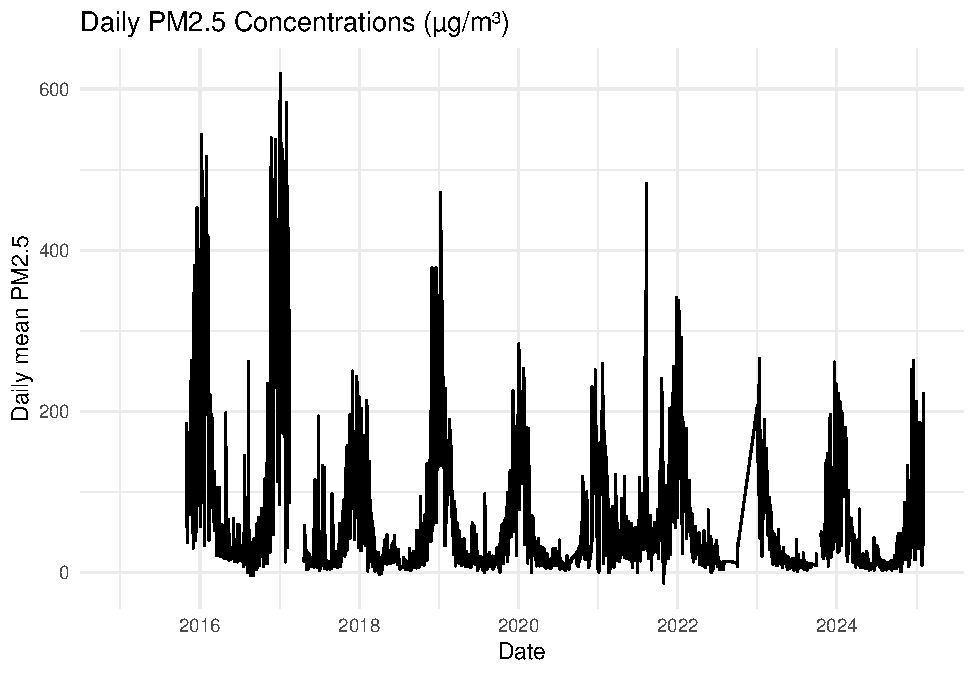
\includegraphics{Project_Report_files/figure-latex/pm25-daily-trend-1.pdf}
\caption{Daily PM2.5 Concentrations (µg/m³)}
\end{figure}

\begin{Shaded}
\begin{Highlighting}[]
\NormalTok{pm25\_yearly\_missing }\OtherTok{\textless{}{-}}\NormalTok{ pm25\_monthly }\SpecialCharTok{\%\textgreater{}\%}
  \FunctionTok{mutate}\NormalTok{(}\AttributeTok{Year =} \FunctionTok{year}\NormalTok{(Month)) }\SpecialCharTok{\%\textgreater{}\%}
  \FunctionTok{group\_by}\NormalTok{(Year) }\SpecialCharTok{\%\textgreater{}\%}
  \FunctionTok{summarize}\NormalTok{(}
    \AttributeTok{total\_months =} \FunctionTok{n}\NormalTok{(),}
    \AttributeTok{months\_with\_missing\_days =} \FunctionTok{sum}\NormalTok{(days\_missing\_raw }\SpecialCharTok{\textgreater{}} \DecValTok{0}\NormalTok{),}
    \AttributeTok{total\_missing\_days =} \FunctionTok{sum}\NormalTok{(days\_missing\_raw),}
    \AttributeTok{.groups =} \StringTok{"drop"}
\NormalTok{  )}

\FunctionTok{ggplot}\NormalTok{(pm25\_yearly\_missing, }\FunctionTok{aes}\NormalTok{(}\AttributeTok{x =}\NormalTok{ Year, }\AttributeTok{y =}\NormalTok{ months\_with\_missing\_days)) }\SpecialCharTok{+}
  \FunctionTok{geom\_col}\NormalTok{(}\AttributeTok{fill =} \StringTok{"tomato"}\NormalTok{) }\SpecialCharTok{+}
  \FunctionTok{labs}\NormalTok{(}
    \AttributeTok{title =} \StringTok{"Number of Months with Missing PM2.5 Data by Year"}\NormalTok{,}
    \AttributeTok{x =} \StringTok{"Year"}\NormalTok{,}
    \AttributeTok{y =} \StringTok{"Months with ≥1 Missing Day"}
\NormalTok{  ) }\SpecialCharTok{+}
  \FunctionTok{theme\_minimal}\NormalTok{()}
\end{Highlighting}
\end{Shaded}

\begin{figure}
\centering
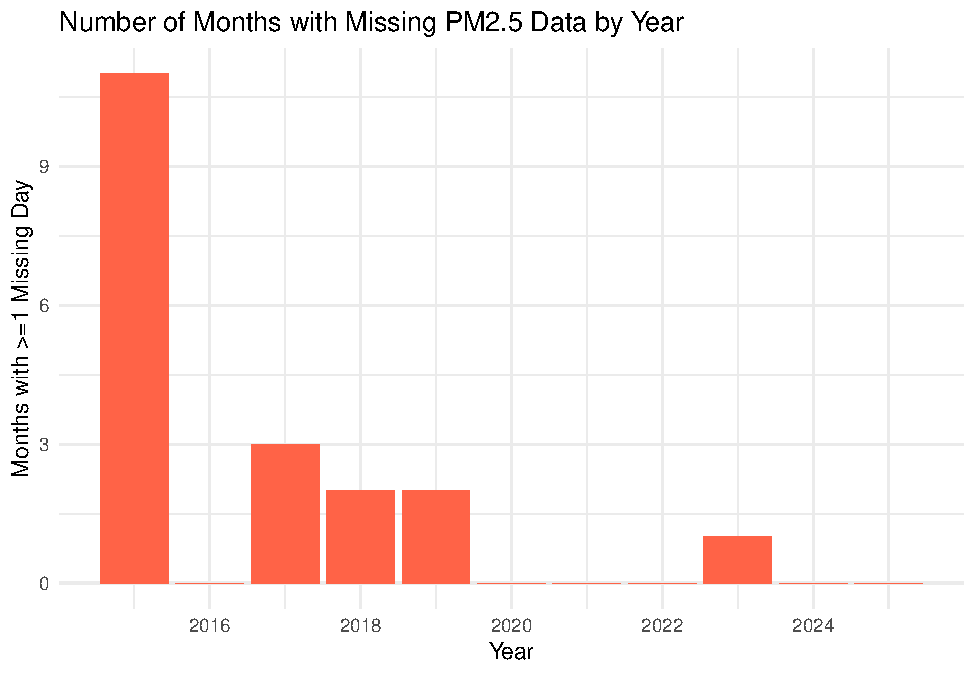
\includegraphics{Project_Report_files/figure-latex/pm25-missing-by-year-1.pdf}
\caption{Number of Months with Missing PM2.5 Data by Year}
\end{figure}

\begin{Shaded}
\begin{Highlighting}[]
\FunctionTok{ggplot}\NormalTok{(pm25\_monthly, }\FunctionTok{aes}\NormalTok{(}\AttributeTok{y =}\NormalTok{ raw\_conc\_monthly)) }\SpecialCharTok{+}
  \FunctionTok{geom\_boxplot}\NormalTok{(}\AttributeTok{outlier.colour =} \StringTok{"red"}\NormalTok{, }\AttributeTok{outlier.shape =} \DecValTok{1}\NormalTok{) }\SpecialCharTok{+}
  \FunctionTok{labs}\NormalTok{(}
    \AttributeTok{title =} \StringTok{"Distribution of Monthly PM2.5"}\NormalTok{,}
    \AttributeTok{y =} \StringTok{"Monthly mean PM2.5 (µg/m³)"}
\NormalTok{  ) }\SpecialCharTok{+}
  \FunctionTok{theme\_minimal}\NormalTok{()}
\end{Highlighting}
\end{Shaded}

\begin{figure}
\centering
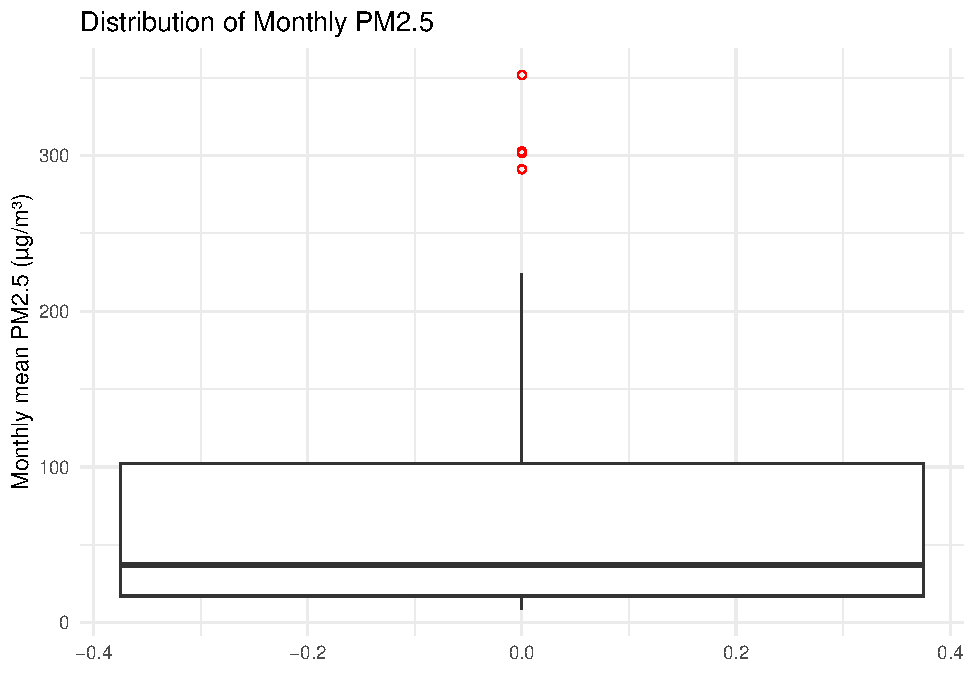
\includegraphics{Project_Report_files/figure-latex/pm25-monthly-boxplot-1.pdf}
\caption{Distribution of Monthly PM2.5 Concentrations}
\end{figure}

\begin{Shaded}
\begin{Highlighting}[]
\CommentTok{\# Compute low birth weight rate (Percentage)}
\NormalTok{full\_data }\OtherTok{\textless{}{-}}\NormalTok{ full\_data }\SpecialCharTok{\%\textgreater{}\%} \FunctionTok{mutate}\NormalTok{(}\AttributeTok{LBW\_rate =} \DecValTok{100} \SpecialCharTok{*}\NormalTok{ Low\_Birth\_Weight }\SpecialCharTok{/}\NormalTok{ Live\_Births)}

\FunctionTok{ggplot}\NormalTok{(full\_data, }\FunctionTok{aes}\NormalTok{(}\AttributeTok{x =}\NormalTok{ raw\_conc\_monthly, }\AttributeTok{y =}\NormalTok{ LBW\_rate)) }\SpecialCharTok{+}
  \FunctionTok{geom\_point}\NormalTok{() }\SpecialCharTok{+}
  \FunctionTok{geom\_smooth}\NormalTok{(}\AttributeTok{method =} \StringTok{"lm"}\NormalTok{, }\AttributeTok{se =} \ConstantTok{TRUE}\NormalTok{, }\AttributeTok{color =} \StringTok{"blue"}\NormalTok{) }\SpecialCharTok{+}
  \FunctionTok{labs}\NormalTok{(}
    \AttributeTok{title =} \StringTok{"Low Birth Weight Rate vs. Monthly PM2.5"}\NormalTok{,}
    \AttributeTok{x =} \StringTok{"PM2.5 (µg/m³)"}\NormalTok{,}
    \AttributeTok{y =} \StringTok{"LBW Rate (Percentage)"}
\NormalTok{  ) }\SpecialCharTok{+}
  \FunctionTok{theme\_minimal}\NormalTok{()}
\end{Highlighting}
\end{Shaded}

\begin{verbatim}
## `geom_smooth()` using formula = 'y ~ x'
\end{verbatim}

\begin{figure}
\centering
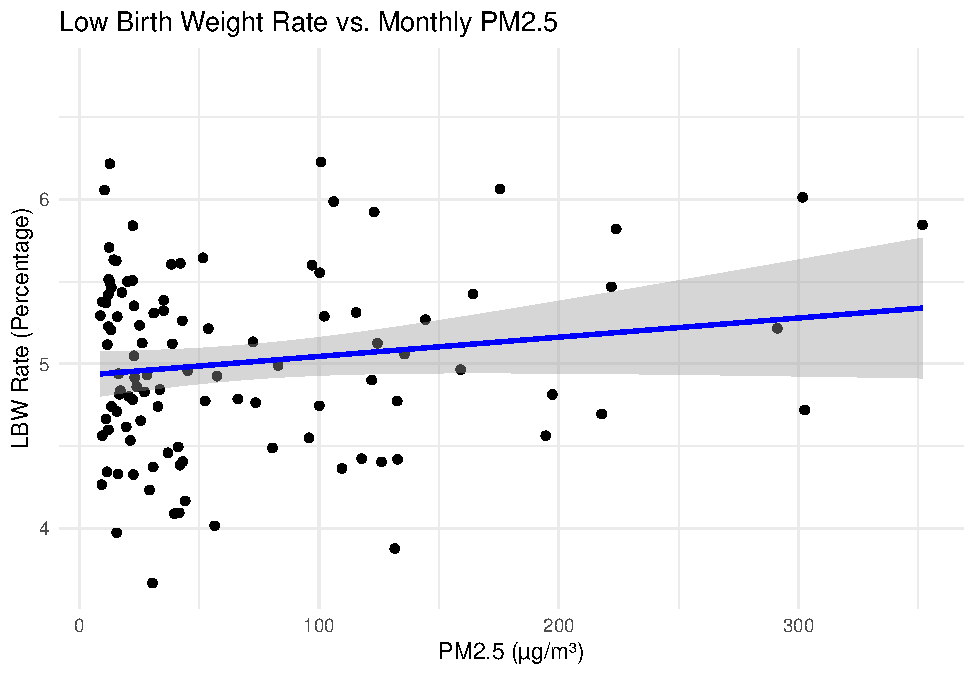
\includegraphics{Project_Report_files/figure-latex/lbw-vs-pm25-1.pdf}
\caption{Low Birth Weight Rate vs.~Monthly PM2.5}
\end{figure}

\begin{Shaded}
\begin{Highlighting}[]
\CommentTok{\# Summary statistics for birth outcomes and PM2.5}
\NormalTok{births\_summary }\OtherTok{\textless{}{-}}\NormalTok{ full\_data }\SpecialCharTok{\%\textgreater{}\%} \FunctionTok{summarise}\NormalTok{(}
  \AttributeTok{Mean\_LBW =} \FunctionTok{mean}\NormalTok{(Low\_Birth\_Weight, }\AttributeTok{na.rm =} \ConstantTok{TRUE}\NormalTok{),}
  \AttributeTok{Median\_LBW =} \FunctionTok{median}\NormalTok{(Low\_Birth\_Weight, }\AttributeTok{na.rm =} \ConstantTok{TRUE}\NormalTok{),}
  \AttributeTok{Min\_LBW =} \FunctionTok{min}\NormalTok{(Low\_Birth\_Weight, }\AttributeTok{na.rm =} \ConstantTok{TRUE}\NormalTok{),}
  \AttributeTok{Max\_LBW =} \FunctionTok{max}\NormalTok{(Low\_Birth\_Weight, }\AttributeTok{na.rm =} \ConstantTok{TRUE}\NormalTok{),}
  \AttributeTok{SD\_LBW =} \FunctionTok{sd}\NormalTok{(Low\_Birth\_Weight, }\AttributeTok{na.rm =} \ConstantTok{TRUE}\NormalTok{),}
  \AttributeTok{N\_LBW =} \FunctionTok{sum}\NormalTok{(}\SpecialCharTok{!}\FunctionTok{is.na}\NormalTok{(Low\_Birth\_Weight)),}
  \AttributeTok{Mean\_Live =} \FunctionTok{mean}\NormalTok{(Live\_Births, }\AttributeTok{na.rm =} \ConstantTok{TRUE}\NormalTok{),}
  \AttributeTok{Median\_Live =} \FunctionTok{median}\NormalTok{(Live\_Births, }\AttributeTok{na.rm =} \ConstantTok{TRUE}\NormalTok{),}
  \AttributeTok{Min\_Live =} \FunctionTok{min}\NormalTok{(Live\_Births, }\AttributeTok{na.rm =} \ConstantTok{TRUE}\NormalTok{),}
  \AttributeTok{Max\_Live =} \FunctionTok{max}\NormalTok{(Live\_Births, }\AttributeTok{na.rm =} \ConstantTok{TRUE}\NormalTok{),}
  \AttributeTok{SD\_Live =} \FunctionTok{sd}\NormalTok{(Live\_Births, }\AttributeTok{na.rm =} \ConstantTok{TRUE}\NormalTok{),}
  \AttributeTok{N\_Live =} \FunctionTok{sum}\NormalTok{(}\SpecialCharTok{!}\FunctionTok{is.na}\NormalTok{(Live\_Births))}
\NormalTok{)}

\NormalTok{pm25\_summary }\OtherTok{\textless{}{-}}\NormalTok{ full\_data }\SpecialCharTok{\%\textgreater{}\%} \FunctionTok{summarise}\NormalTok{(}
  \AttributeTok{Mean\_PM25 =} \FunctionTok{mean}\NormalTok{(raw\_conc\_monthly, }\AttributeTok{na.rm =} \ConstantTok{TRUE}\NormalTok{),}
  \AttributeTok{Median\_PM25 =} \FunctionTok{median}\NormalTok{(raw\_conc\_monthly, }\AttributeTok{na.rm =} \ConstantTok{TRUE}\NormalTok{),}
  \AttributeTok{Min\_PM25 =} \FunctionTok{min}\NormalTok{(raw\_conc\_monthly, }\AttributeTok{na.rm =} \ConstantTok{TRUE}\NormalTok{),}
  \AttributeTok{Max\_PM25 =} \FunctionTok{max}\NormalTok{(raw\_conc\_monthly, }\AttributeTok{na.rm =} \ConstantTok{TRUE}\NormalTok{),}
  \AttributeTok{SD\_PM25 =} \FunctionTok{sd}\NormalTok{(raw\_conc\_monthly, }\AttributeTok{na.rm =} \ConstantTok{TRUE}\NormalTok{),}
  \AttributeTok{N\_PM25 =} \FunctionTok{sum}\NormalTok{(}\SpecialCharTok{!}\FunctionTok{is.na}\NormalTok{(raw\_conc\_monthly)),}
  \AttributeTok{Mean\_AQI =} \FunctionTok{mean}\NormalTok{(aqi\_monthly, }\AttributeTok{na.rm =} \ConstantTok{TRUE}\NormalTok{),}
  \AttributeTok{Median\_AQI =} \FunctionTok{median}\NormalTok{(aqi\_monthly, }\AttributeTok{na.rm =} \ConstantTok{TRUE}\NormalTok{),}
  \AttributeTok{Min\_AQI =} \FunctionTok{min}\NormalTok{(aqi\_monthly, }\AttributeTok{na.rm =} \ConstantTok{TRUE}\NormalTok{),}
  \AttributeTok{Max\_AQI =} \FunctionTok{max}\NormalTok{(aqi\_monthly, }\AttributeTok{na.rm =} \ConstantTok{TRUE}\NormalTok{),}
  \AttributeTok{SD\_AQI =} \FunctionTok{sd}\NormalTok{(aqi\_monthly, }\AttributeTok{na.rm =} \ConstantTok{TRUE}\NormalTok{),}
  \AttributeTok{N\_AQI =} \FunctionTok{sum}\NormalTok{(}\SpecialCharTok{!}\FunctionTok{is.na}\NormalTok{(aqi\_monthly))}
\NormalTok{)}

\CommentTok{\# Summary tables}
\NormalTok{births\_summary }\SpecialCharTok{\%\textgreater{}\%}
  \FunctionTok{t}\NormalTok{() }\SpecialCharTok{\%\textgreater{}\%} \FunctionTok{as.data.frame}\NormalTok{() }\SpecialCharTok{\%\textgreater{}\%}
  \FunctionTok{rownames\_to\_column}\NormalTok{(}\StringTok{"Statistic"}\NormalTok{) }\SpecialCharTok{\%\textgreater{}\%}
  \FunctionTok{rename}\NormalTok{(}\AttributeTok{Value =}\NormalTok{ V1) }\SpecialCharTok{\%\textgreater{}\%}
  \FunctionTok{kable}\NormalTok{(}\AttributeTok{caption =} \StringTok{"Summary of Birth Outcomes"}\NormalTok{, }\AttributeTok{digits =} \DecValTok{2}\NormalTok{) }\SpecialCharTok{\%\textgreater{}\%}
  \FunctionTok{kable\_styling}\NormalTok{(}\AttributeTok{full\_width =} \ConstantTok{FALSE}\NormalTok{)}
\end{Highlighting}
\end{Shaded}

\begin{longtable}[t]{lr}
\caption{\label{tab:summary-statistics}Summary of Birth Outcomes}\\
\toprule
Statistic & Value\\
\midrule
Mean\_LBW & 155.97\\
Median\_LBW & 153.00\\
Min\_LBW & 88.00\\
Max\_LBW & 214.00\\
SD\_LBW & 21.87\\
\addlinespace
N\_LBW & 111.00\\
Mean\_Live & 3110.86\\
Median\_Live & 3187.00\\
Min\_Live & 1934.00\\
Max\_Live & 3737.00\\
\addlinespace
SD\_Live & 360.42\\
N\_Live & 111.00\\
\bottomrule
\end{longtable}

\begin{Shaded}
\begin{Highlighting}[]
\NormalTok{pm25\_summary }\SpecialCharTok{\%\textgreater{}\%}
  \FunctionTok{t}\NormalTok{() }\SpecialCharTok{\%\textgreater{}\%} \FunctionTok{as.data.frame}\NormalTok{() }\SpecialCharTok{\%\textgreater{}\%}
  \FunctionTok{rownames\_to\_column}\NormalTok{(}\StringTok{"Statistic"}\NormalTok{) }\SpecialCharTok{\%\textgreater{}\%}
  \FunctionTok{rename}\NormalTok{(}\AttributeTok{Value =}\NormalTok{ V1) }\SpecialCharTok{\%\textgreater{}\%}
  \FunctionTok{kable}\NormalTok{(}\AttributeTok{caption =} \StringTok{"Summary of Monthly PM2.5 Exposure"}\NormalTok{, }\AttributeTok{digits =} \DecValTok{2}\NormalTok{) }\SpecialCharTok{\%\textgreater{}\%}
  \FunctionTok{kable\_styling}\NormalTok{(}\AttributeTok{full\_width =} \ConstantTok{FALSE}\NormalTok{)}
\end{Highlighting}
\end{Shaded}

\begin{longtable}[t]{lr}
\caption{\label{tab:summary-statistics}Summary of Monthly PM2.5 Exposure}\\
\toprule
Statistic & Value\\
\midrule
Mean\_PM25 & 67.28\\
Median\_PM25 & 35.22\\
Min\_PM25 & 8.80\\
Max\_PM25 & 351.76\\
SD\_PM25 & 72.90\\
\addlinespace
N\_PM25 & 107.00\\
Mean\_AQI & 111.86\\
Median\_AQI & 92.67\\
Min\_AQI & 31.73\\
Max\_AQI & 274.00\\
\addlinespace
SD\_AQI & 66.15\\
N\_AQI & 107.00\\
\bottomrule
\end{longtable}

\newpage

\section{Analysis}\label{analysis}

\newpage

\section{Results and Interpretation}\label{results-and-interpretation}

\newpage

\section{Conclusion and Policy
Implications}\label{conclusion-and-policy-implications}

\newpage

\section{References}\label{references}

\end{document}
